\section{Experiments}
\begin{figure}
  \centering
  \begin{subfigure}[b]{0.48\linewidth}
    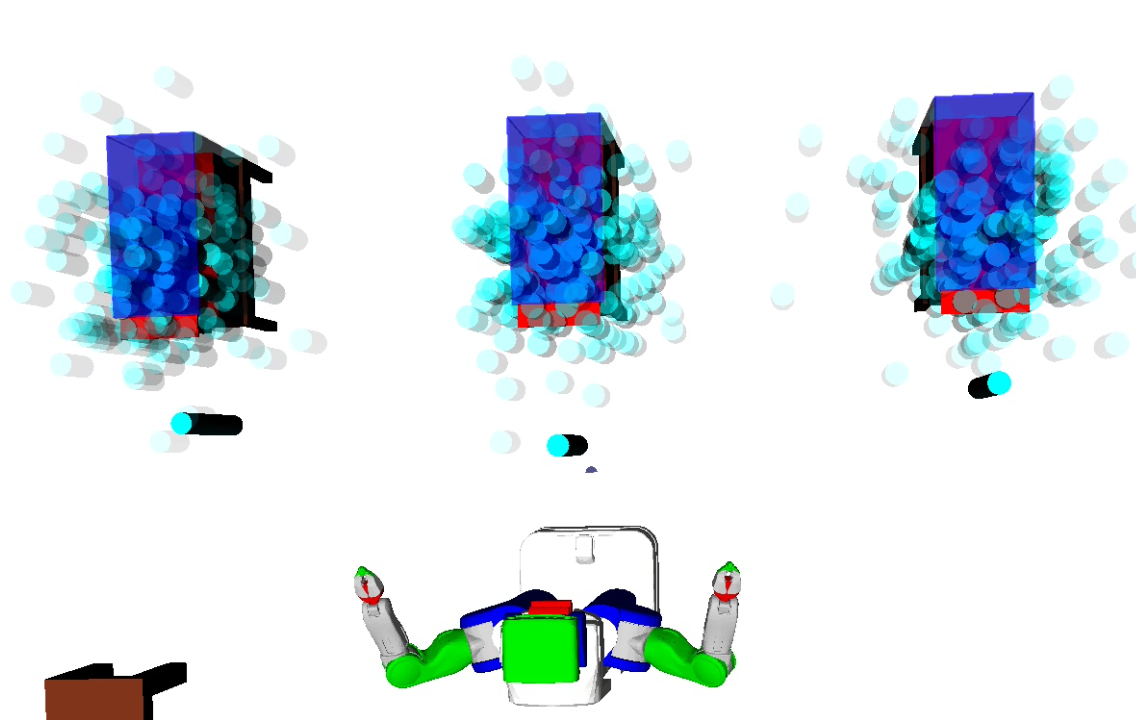
\includegraphics[width=\textwidth]{drawer_images/drawer_dist_0.png}
    \caption{}
    \label{fig:step1}
  \end{subfigure}
  \begin{subfigure}[b]{0.48\linewidth}
    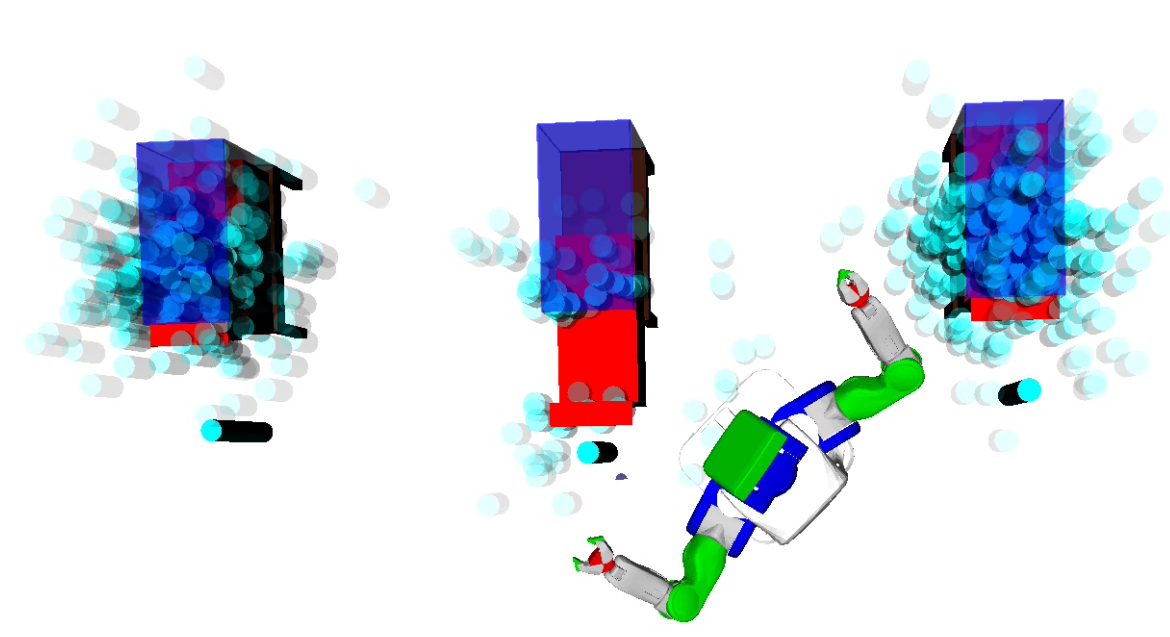
\includegraphics[width=\textwidth]{drawer_images/drawer_dist_1.png}
    \caption{}
    \label{fig:step2}
  \end{subfigure}
  \begin{subfigure}[b]{0.48\linewidth}
    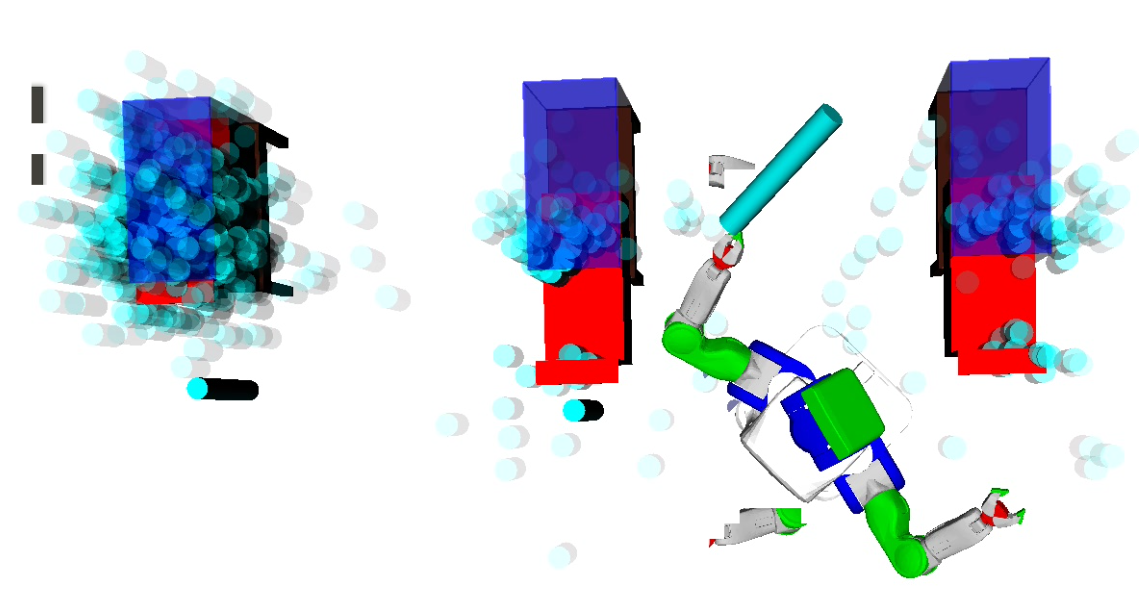
\includegraphics[width=\textwidth]{drawer_images/drawer_dist_2.png}
    \caption{}
    \label{fig:step4}
  \end{subfigure}
  \begin{subfigure}[b]{0.48\linewidth}
    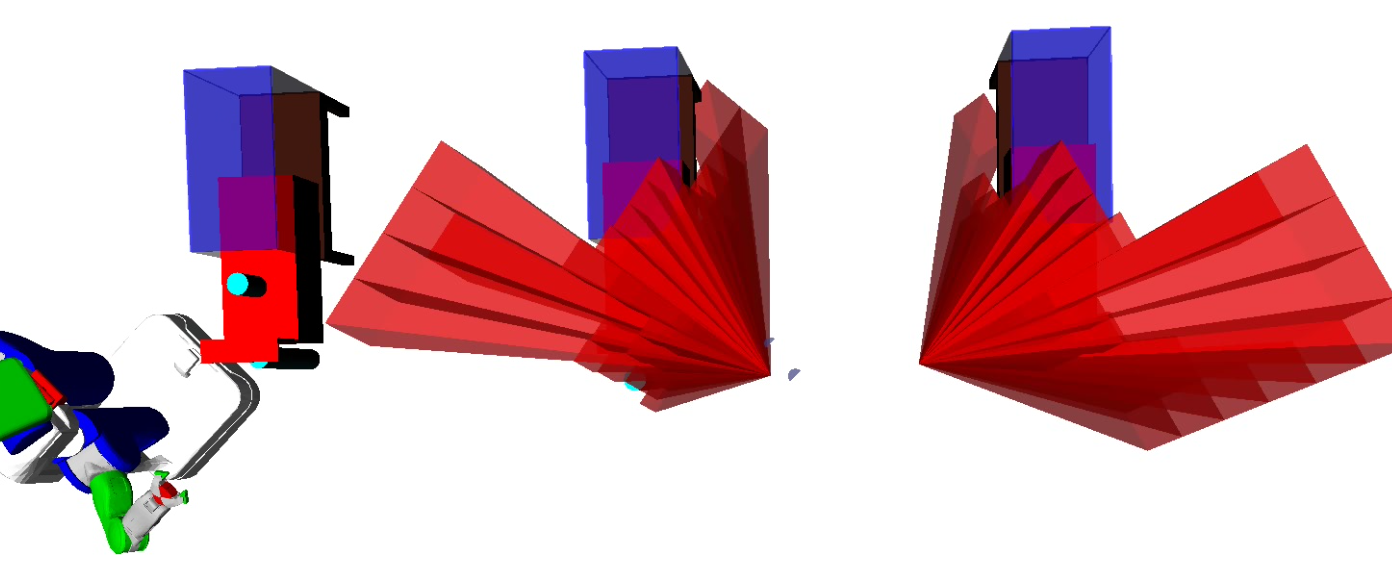
\includegraphics[width=\textwidth]{drawer_images/drawer_dist_negreg.png}
    \caption{}
    \label{fig:step5}
  \end{subfigure}
  %% \begin{subfigure}[b]{0.3\linewidth}
  %%   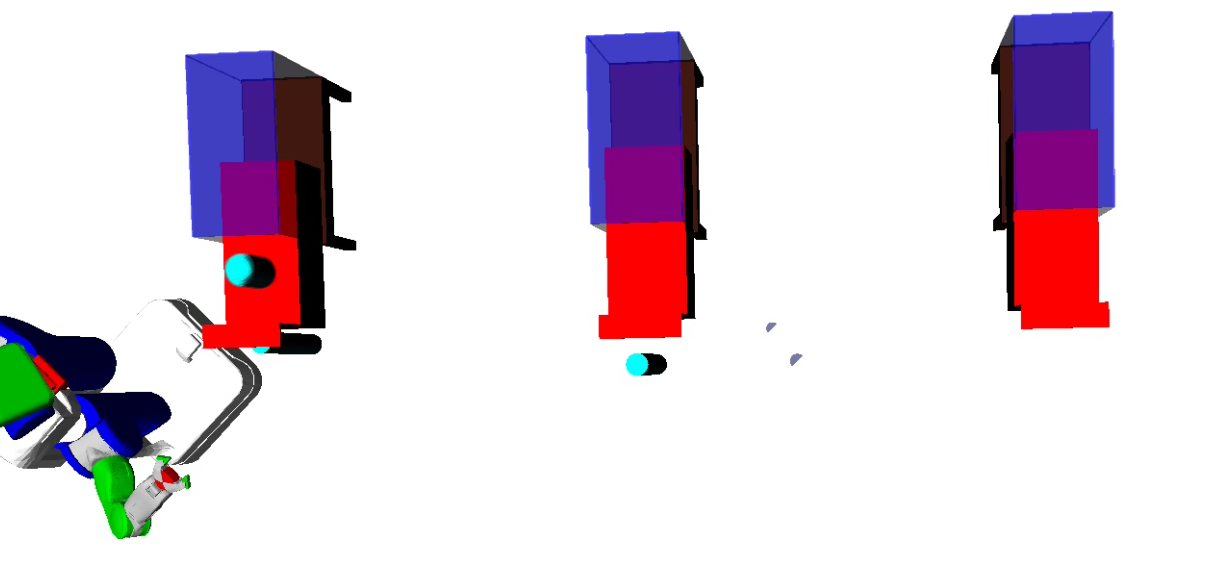
\includegraphics[width=\textwidth]{drawer_images/drawer_dist_3.png}
  %%   \caption{After observing three drawers (object was seen)}
  %%   \label{fig:step6}
  %% \end{subfigure}
  \caption{Intermediate belief states from a sample execution in our
    drawer search domain. We search for an object with a multimodal
    Gaussian distribution over three drawers. We illustrate beliefs with
    samples from the posterior distribution and show likelihoods with
    the transparency of objects. In this case, the object was in the
    leftmost drawer, and was found after searching the other
    drawers because they had a higher likelihood of containing the object. (a) shows the initial state and (b) and (c) show
    intermediate states at which we had to replan. Notice that we only clear
    the obstruction in front of the drawer when it is close enough to hinder sufficient opening.
    (d) shows the view cones from negative observations that were generated during planning.}
  \label{fig:drawerimgs}
\end{figure}

\begin{figure*}
  \centering
  \begin{subfigure}[b]{0.22\linewidth}
    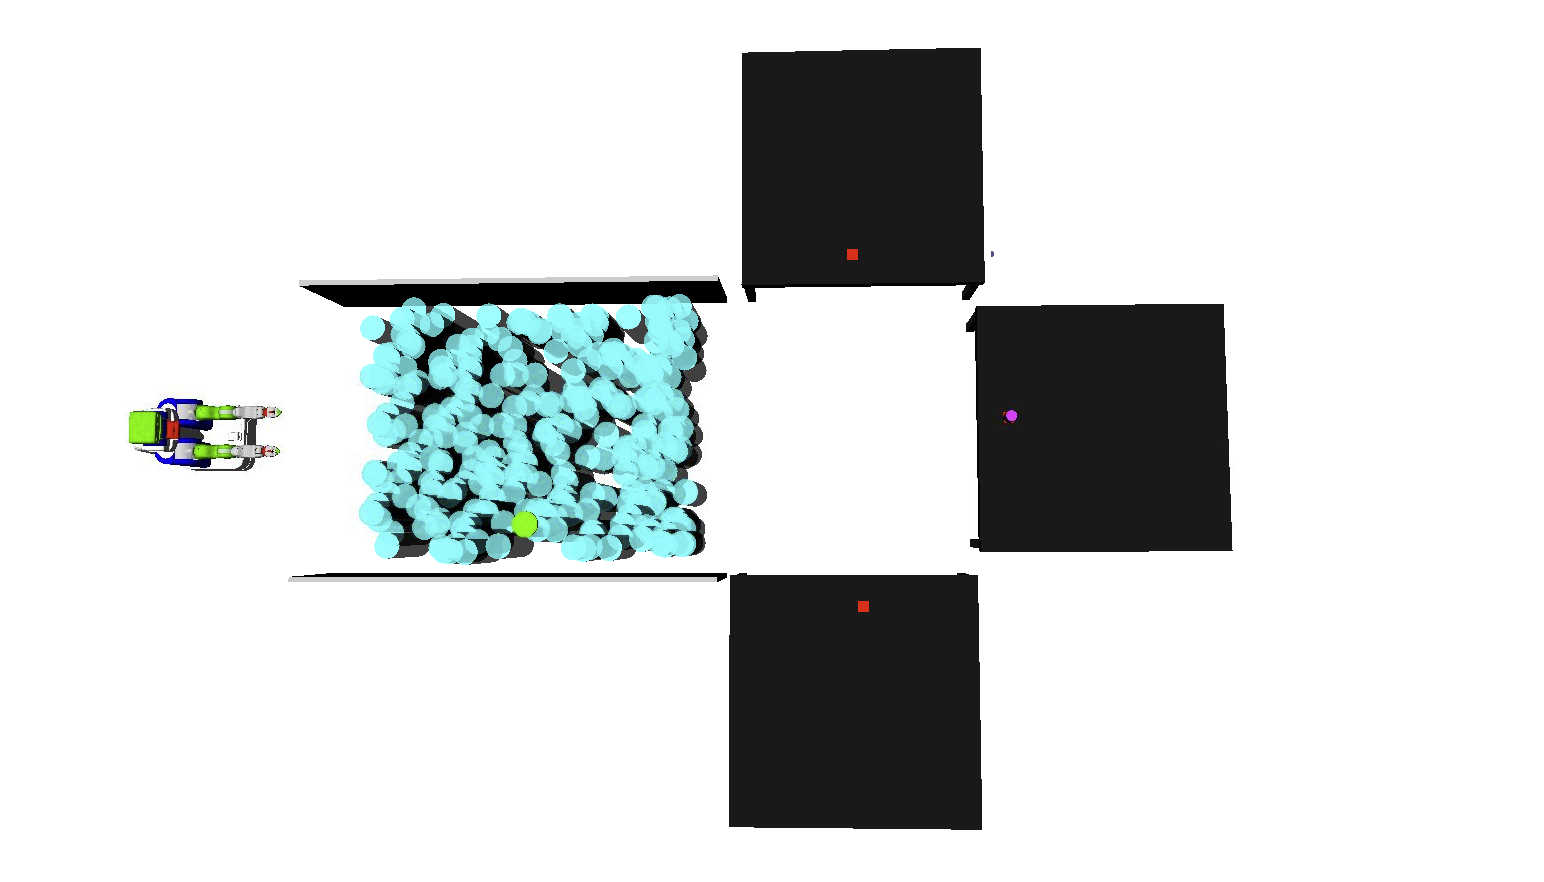
\includegraphics[width=\textwidth]{corridor_images/0-observe.png}
    \caption{Initial belief state}
    \label{fig:step1}
  \end{subfigure}
  \begin{subfigure}[b]{0.22\linewidth}
    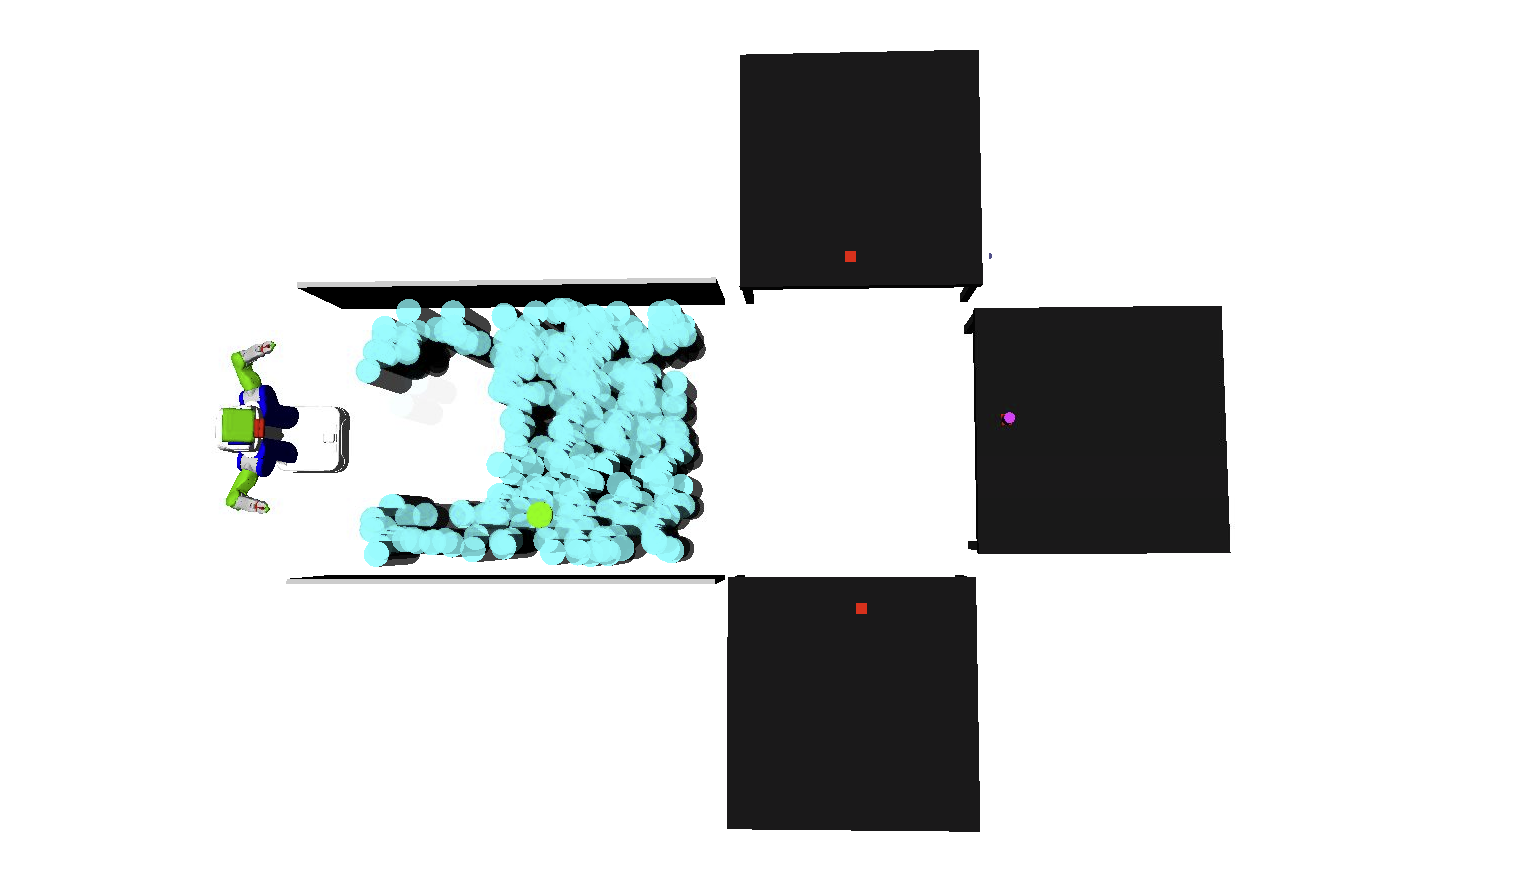
\includegraphics[width=\textwidth]{corridor_images/1-observe.png}
    \caption{After 1 observations}
    \label{fig:step2}
  \end{subfigure}
  \begin{subfigure}[b]{0.22\linewidth}
    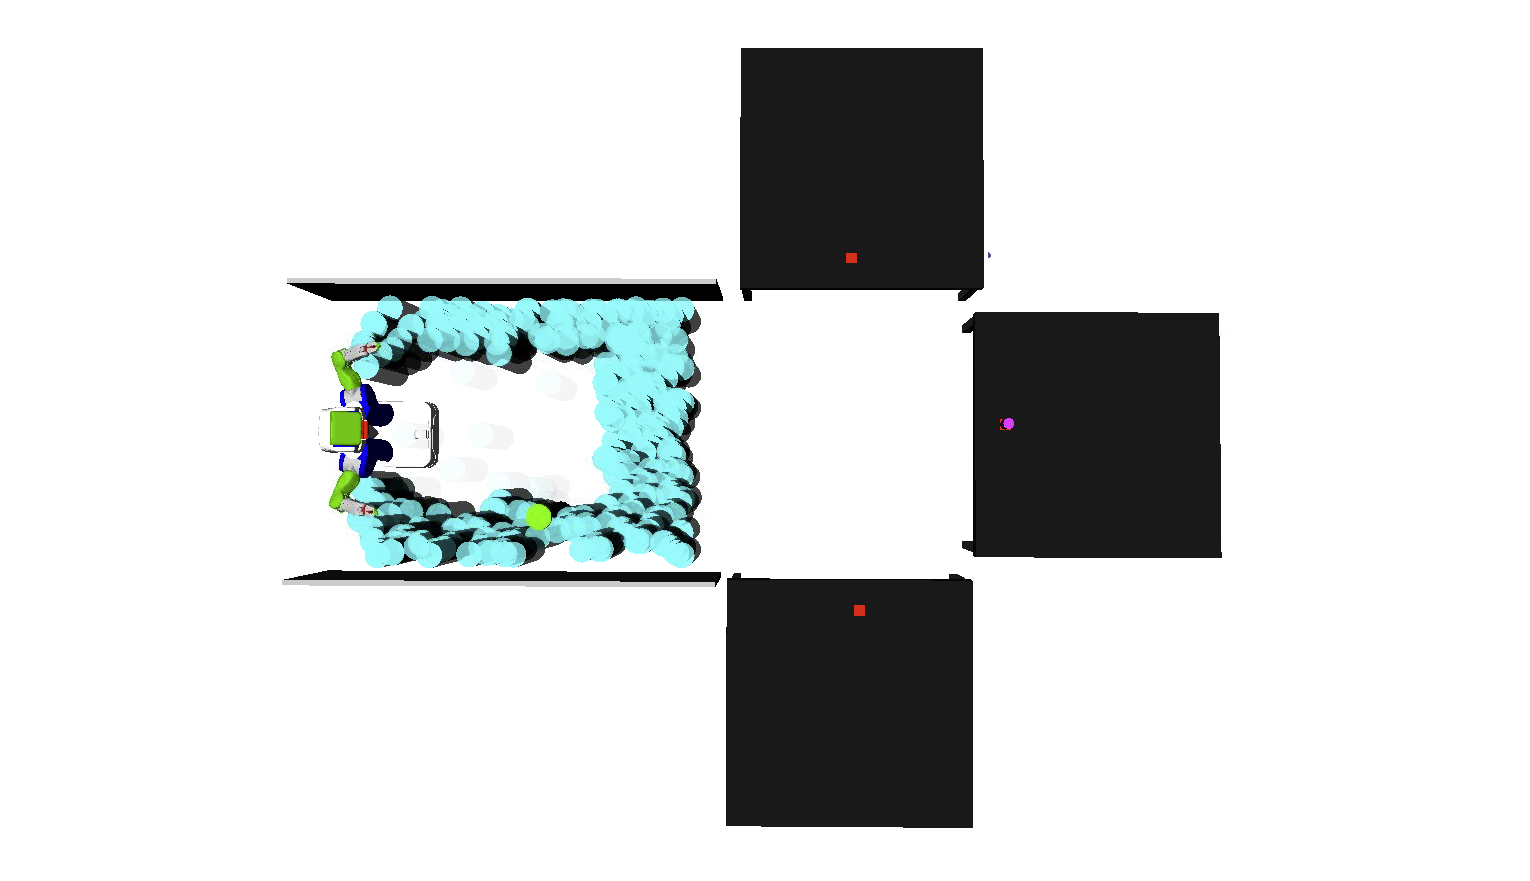
\includegraphics[width=\textwidth]{corridor_images/2-observe.png}
    \caption{After 2 observations}
    \label{fig:step3}
  \end{subfigure}
  \begin{subfigure}[b]{0.22\linewidth}
    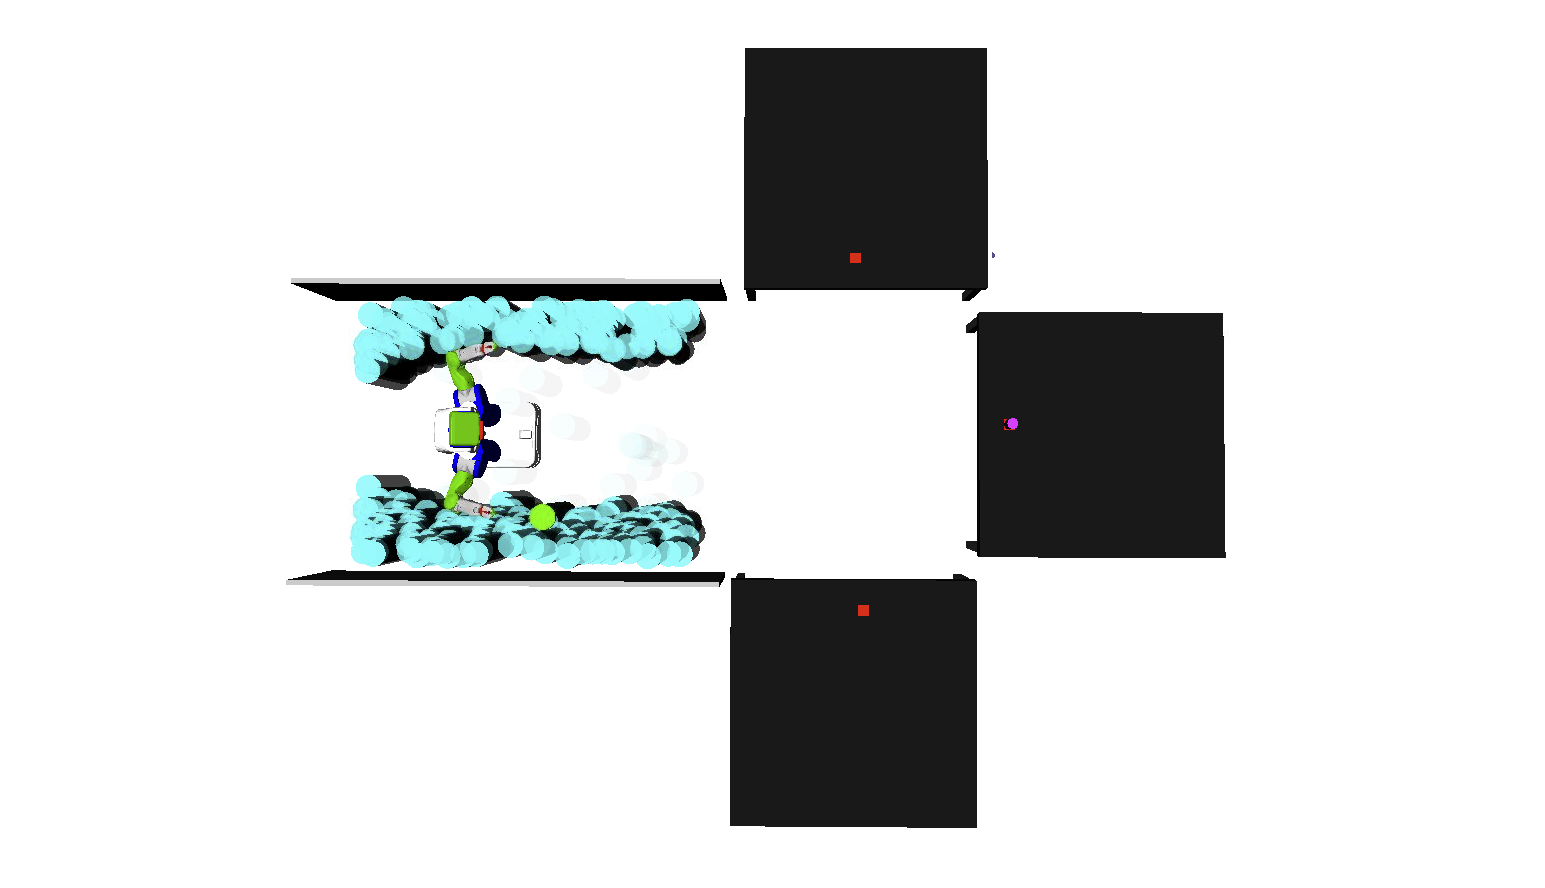
\includegraphics[width=\textwidth]{corridor_images/3-observe.png}
    \caption{After 3 observations}
    \label{fig:step4}
  \end{subfigure}
  \caption{Execution trace of interfaced belief space planning
    traversing a corridor with uncertain obstacles.
    The blue cylinders are drawn from the uniform belief distribution
    during execution. After reaching the other side of the corridor,
    the robot will pick up two target tables from the three tables.}
  \label{fig:corridorimgs}
\end{figure*}

We evaluate \ibsp{} in partially observable pick-and-place and navigation tasks.
The robot in our simulation is a full model of the Willow Garage PR2. We
provide results for several belief distributions: unimodal Gaussian, multimodal
Gaussian, and uniform.
\subsection{Observation Operator Specification and Generators}
The maximum likelihood component of the determinized problem
essentially follows the dynamics specified in
\secref{sec-formulation}. In order to extend this domain to handle
partial observability, we add the following fluents and operators:
\begin{tightlist}
  \item[]Fluents: \\\emph{MLInView}(r\_pose, o\_pose\_bel)\\
    \emph{MLOccludes}(obj, o\_pose\_bel, r\_obs\_pose)\\
    \emph{MLObstructs}(obj, traj)\\
    \emph{UncertainGP}(o\_pose\_bel, r\_pose, grasp)\\
    \emph{UncertainObstructs}(obj, traj)
  \item[]Operators:
  \begin{tightlist} \item \emph{ObserveGP}(r\_obs\_pose, o, o\_pose\_bel)
\begin{tightlist}
  \item[\emph{pre}:] \emph{MLLoc}(o, o\_pose\_bel) $\wedge$
    \emph{MLRLoc}(r\_obs\_pose) \\$\wedge$ $\forall o_i
    \lnot$\emph{MLOccludes}($o_i$, o\_pose\_bel, r\_obs\_pose) \\ $\wedge$
    \emph{MLInView}(r\_obs\_pose, o\_pose)
  \item[\emph{eff}:] $\forall$ r\_p, g $\lnot$\emph{UncertainGP}(o\_pose\_bel, r\_p, g)
\end{tightlist}
\item  \emph{ObserveTrajectory}(r\_obs\_pose, traj) 

\begin{tightlist}
  \item[\emph{pre}:] \emph{MLRLoc}(r\_obs\_pose) \\$\wedge$
    \emph{MLInView}(r\_obs\_pose, traj)\\ $\wedge$
    $\forall o_i \lnot$\emph{MLOccludes}($o_i$, traj, r\_obs\_pose)\\ $\wedge$
    $\forall o_i \lnot$\emph{MLObstructs}(obj, traj)
  \item[\emph{eff}:] $\forall o_i \lnot$\emph{UncertainObstructs}($o_i$,
    traj)
\end{tightlist}
\end{tightlist}
\end{tightlist}

The additional skolem functions needed to support this functionality
are \emph{ViewPose}(Obj) and \emph{ViewPose}(Traj) for each object and
trajectory reference. The generator for object view poses draws
samples from a 1-meter unit disc around the object, and the head pose
is fixed to point at the object's maximum likelihood position. The
generator for trajectory view poses returns the first step along the
trajectory that has non-negligible probability of being in
collision. To observe the uncertain step, a viable base pose is
sampled from regions with negligible collision probability along the
same trajectory.

\subsection{Observation model and state estimation for the PR2}
We model observations with ray casting from a simulated head-mounted
Kinect on our robot. For objects that are in the view
frustum, we get a false negative with probability proportional to the
amount of the object that is occluded. If we do get a positive
observation, we observe the object's true pose with Gaussian noise.


In order to successfully plan for this domain, it is important that we
effectively incorporate negative observations into our
updates. Without these negative observations, it is impossible to determine
if a trajectory is clear without observing actual objects
locations. 

We account for negative observations with a factored representation
for the belief state. In one component, we maintain a distribution
that accounts for positive observations (e.g., a Kalman filter). The
other component is an explicit representation of the view cones
associated with negative observations. We refer to the first component
as the positive observation distribution and the second as the
negative regions. To sample from this distribution, we perform
probabilistic rejection sampling: sample from the positive observation
distribution and then discard the sample in inverse proportion to the
probability that it lies in a negative region. The inverse
probability is given by $\max(1,\dfrac{\text{penetration
    depth}}{\text{object radius}})$, where penetration depth is the
minimum translation distance that takes two objects out of collision and object
radius is found by approximating the object as a sphere.


\subsection{Evaluations}
We implement our experiments in Python and use
OpenRave~\cite{Diankov_2008_6117} to represent the environment. We use
trajectory optimization for our motion planning~\cite{schulman2013finding}
and implement custom collision checking in Flexible Collision Library~\cite{jia2014fcl} to handle
collisions. We use the Fast-Forward and Fast-Downward
task planners to solve our high-level planning problems. Because our system works
independently of the chosen task planner, we use Fast-Forward in domains involving negative
preconditions, which are not supported by Fast-Downward. Experiments were run in series on
Intel Core i7-4770K machines with 16GB RAM. We validate our approach in three distinct scenarios.

To explore ensuring safety in robot navigation tasks under uncertainty, we
evaluate performance in a corridor domain. We place the robot at one end of a corridor
and present it with the goal of traversing the corridor, then grasping
objects on tables on the other side. Uniform distributions model the locations of
a varying number of obstructing columns throughout the corridor; thus, the solution
typically ends up as an alternating sequence of observations and motions. Note that this task would be essentially
insoluble without accounting for negative observations appropriately.

The second task demonstrates the ability to reason about occlusions. We
set a goal of grasping a target object from a cluttered table with other
objects on it: some have deterministic locations and others have a Gaussian distribution
modeling their location. The target object's location is also drawn from a Gaussian
distribution. \ibsp{} plans to remove any occlusions, to observe the target object, and
then to pick it up. In our experiments, we maintain that 3 of the objects on the table -- always including
the target object -- are part of the belief space.

In our final scenario, the robot has lost its keys and is trying to locate them among three drawers they could be in.
This setup illustrates multimodal planning behavior with a mixture of Gaussians as the prior for the target's location.
Furthermore, we introduce a deterministic object in front of each drawer, which possibly
obstructs it from being opened. \ibsp{} begins by assuming the target is placed at its maximum likelihood
location; accordingly, it discovers that the target is obstructed by the drawer containing it, then
plans to open this drawer. If the outer deterministic object impedes the drawer from opening, this
obstruction fact is also discovered and accounted for. During execution, upon performing an observation inside the drawer, our system
chooses to refine the plan if the object was not actually seen (indicating that its true location is in another drawer).
The new refinement incorporates this negative observation, and the system may then try opening another drawer.

Table \ref{table:results} shows timing results for the three described
tasks. \figref{fig:drawerimgs} and \figref{fig:corridorimgs} show intermediate steps and belief
states for the drawer and corridor tasks. The included video demonstrates plan execution for all three tasks.


\begin{table}
  \centering
  \vspace{8pt}
  \tabcolsep=0.11cm{
  \begin{tabular}{cccc}
    \toprule
      Problem Type & \% Solved & Avg Time (s) & Avg \# Planner Runs\\
    \midrule
      Uni. corridor, 1 obj & 100 & 232 & 1.88\\
    \midrule
      Uni. corridor, 2 obj & 100 & 445 & 2.45\\
    \midrule
      Uni. corridor, 3 obj & 88 & 926 & 2.78\\
    \midrule
      Uni. corridor, 4 obj & 58 & 1168 & 2\\
    \midrule
      Table, 5 obj & 95 & 89 & 2.2\\
    \midrule
      Table, 10 obj & 95 & 162 & 2.21\\
    \midrule
      Table, 15 obj & 83 & 135 & 2.26\\
    \midrule
      Table, 20 obj & 70 & 229 & 2.03\\
    \midrule
      Table, 25 obj & 68 & 166 & 1.84\\
    \midrule
      Table, 30 obj & 48 & 122 & 1.96\\
    \midrule
      3-Drawer search & 93 & 325 & 2.11\\
    \bottomrule
  \end{tabular}}
  \caption{Solution percentages, running times, and number of high-level planner calls for \ibsp{} in
    occluded search and navigation tasks. Unimodal cluttered table results are from 40
    randomly generated problems per number of objects. Multimodal 3-drawer search results
    are from 30 iterations. Uniform corridor navigation results are from 40 random locations of corridor obstructions, per number of objects. Time limit: 1800s.}
  \label{table:results}
\end{table}



